\usetikzlibrary{arrows.meta}
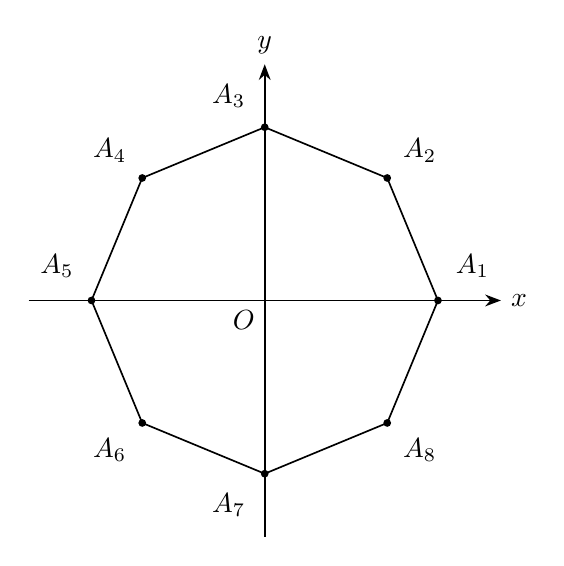
\begin{tikzpicture}[x=1cm,y=1cm,line width=.6pt,font=\normalsize,>=Stealth]
% axes (extend beyond vertices at +-2.2)
\draw[->] (-3.0,0)--(3.0,0) node[right] {$x$};
\draw[->] (0,-3.0)--(0,3.0) node[above] {$y$};
\node[below left] at (0,0) {$O$};
% regular octagon, unit circle scaled by 2.2
\coordinate (A1) at (2.2,0.0);
\coordinate (A2) at (1.5556,1.5556);
\coordinate (A3) at (0.0,2.2);
\coordinate (A4) at (-1.5556,1.5556);
\coordinate (A5) at (-2.2,0.0);
\coordinate (A6) at (-1.5556,-1.5556);
\coordinate (A7) at (0.0,-2.2);
\coordinate (A8) at (1.5556,-1.5556);
\draw (A1)--(A2)--(A3)--(A4)--(A5)--(A6)--(A7)--(A8)--cycle;
% vertex labels in outer whitespace (axis vertices lifted off axis)
\node[above right] at (2.30,0.16) {$A_1$};
\node[above right] at (1.63,1.63) {$A_2$};
\node[above left] at (-0.12,2.32) {$A_3$};
\node[above left] at (-1.63,1.63) {$A_4$};
\node[above left] at (-2.30,0.16) {$A_5$};
\node[below left] at (-1.63,-1.63) {$A_6$};
\node[below left] at (-0.12,-2.32) {$A_7$};
\node[below right] at (1.63,-1.63) {$A_8$};
\fill (A1) circle[radius=1.4pt];
\fill (A2) circle[radius=1.4pt];
\fill (A3) circle[radius=1.4pt];
\fill (A4) circle[radius=1.4pt];
\fill (A5) circle[radius=1.4pt];
\fill (A6) circle[radius=1.4pt];
\fill (A7) circle[radius=1.4pt];
\fill (A8) circle[radius=1.4pt];
\end{tikzpicture}
